\documentclass[10pt,a4paper]{article}
\usepackage[]{hyperref}
\usepackage{graphicx}
\usepackage{array}
\graphicspath{ {./images/} }
\author{Vinko Lovrenčić \\ \footnotesize Mentor: prof. dr. sc. Luka Grubišić \\ Prirodoslovno-matematički fakultet, Matematički odsjek}
\date{February 25th 2021.}
\title{User documentation for using Hill climbing algorithms to solve N-queen problem}
\begin{document}
	\begin{titlepage}
                \maketitle
        \end{titlepage}
	\tableofcontents
	\pagebreak
	\section{Introduction}
		Hill climbing algorith is a local algorithm used for finding a peak of the "mountain" where in each step (state) you find an "step" (called neighbour) towards the peak and take it, until you can't find any more steps: that's when you reach the peak. \\
		Mathematically, hill climbing take a function $f(v)$, where v is some vector and changes one of the vector elements. After that it calculates if the change increased $f(v)$, and if it did it makes the change to $v$ permanent. The algorith repeats until it cannot find a change to $v$ that would increase $f(v)$. That when we say we reach a LOCAL optima.\\
		Some of the characteristics of it are:
		\begin{itemize}
			\item It goes from state to state and compares their values.
			\item We dont have to maintain the search space anywhere since we go from state to state: every new state in calculated from the last one.
			\item It uses a greedy approach: it looks for moves that improve it's cost
			\item Needs a good heuristic: if we dont have it it will be really inefficient and the optimizations will be miniscule
			\item It's an anytime algorithm: it can be interrupted at any time during it's execution and it will give a valid solution
		\end{itemize}
		The goal of the algorithm is to find the GLOBAL optima: the optimization of the problem, whether thats a minimum or a maximum.
	\pagebreak
	\section{Caveats and solutions (or attempts at them)}
		This algorithm has multiple caveats where it can get stuck, or return a value that isn't the best.
		\begin{figure}[h]
			\caption{Possible states in hill climbing}
			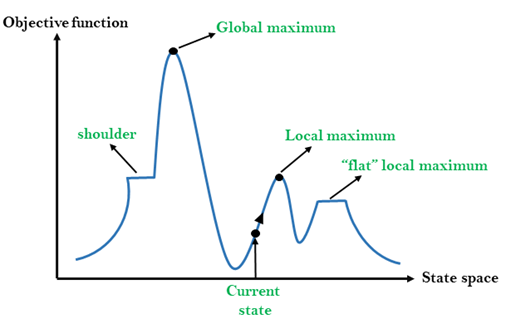
\includegraphics{hill_climbing_graph.png}
			\centering
		\end{figure}
		From left to right we can explain states and problem with them:
		\begin{itemize}
			\item Shoulder is a part of the graph where the graph is rising and then suddenly becomes flat, only to rise again a bit later. The problem here is that if steps arent large enough we can get stuck in a shoulder, thinking either that we reached the optimum (we can't see any improvement in neighbours).
			\item Global maximum (optimum)is the thing we are looking for: hopefully we reach it at the end of our algorithm.
			\item Current state is where we are currently: we examine it's neigbours and go to a better state
			\item Local maximums (optimims) are the biggest enemy of the Hill climbing algorithm: when we reach it our algorithm will think it has reach an optimal solution and it will terminate - after all, every neighbour is a worse state then the current one. 
			\item Flat local maximum (optimum) is an even bigger problem, because not only that ourm algorithm could think that it has reach the optimum, i could get stuck infinitely wandering the plains, hoping to find a solution.
		\end{itemize}
		There are multiple solutions proposed to thiese problems, but here we are going to mainly focus on three of them:
		\begin{enumerate}
			\item Random neighbour: when we reach a shoulder or a local optimum we jump to a random neighbour, even if it's worse then the current one, hoping to jump out of the problematic state. \\
				This approach works when there are a lot more shoulders in the graph than there are local optimas, because it will eventually escape the shoulder, no matter how big of a step it's taking, but it has a lower chance of escaping the local optima, because i till often climb right back to it.
			\item Random restart: when we reach a shoulder or a local optimum we restart the process, basically starting the hill climb again with another, random, starting point, hoping to get a better result this time. \\
				This approach will eventually find the global optimum, and it can equally escape both shoulders and local optima, but it's a lot more processor intensive, so the first approach is preffered if it's conditions (a lot more shoulders than optima) are met. Of course, we could combine them in some way (for instance, use 1. for shoulders and 2. for optima) to get an even better algorithm
			\item Stochastic climbing: we pick a random neighbour of our state and decide with some probability whether we are going to take that step or evaluate another. Of course, we have to value higher improvements more than lower improvement or even regressions (if we don't we aren't really hill climbing anymore, we are just random searching), but we don't exclude those lower improvements or regeresions, we even give them a chance to be picked.//
				Doing this we will eventually escape out of optimas and shoulders, but still we will be chimbing.
		\end{enumerate}
		Of course, there is no best solution, only thing we can do is apply the appropriate one to the problem at hand.
	\pagebreak
	\section{Algorithms}
		Here we are going to be looking at 6 different approaches to the hill climbing algorithm, pros and cons of each one of them, motivation and how the stand up to each other.
		\begin{enumerate}
			\item Simple hill climbing \\
				This is as basic as hill climbing gets: look at neighbours, pick the first one you notice that is better then the current state, move to that state. If we can't find such neighbour we are done.\\
				Pros:
				\begin{itemize}
					\item Faster than most hill climbing algorithms
					\item Will always give a solution, every step will give a better solution
					\item If the graph is convex with small or no shoulder it is incredibly fast and reliable
				\end{itemize}
				Cons:
				\begin{itemize}
                                        \item If the problem graph isn't convenient for it it won't give an optimal solution a lot of the time
					\item Will get stuck in most shoulders and local optimas (only if it can step over them it won't)
                                \end{itemize}
			\item Steepest hill climbing \\
				This is a change to simple alorithm in a way the, instead of looking for the first better neighbour and taking it we look at all possible neighbours and take the best (the steepest) one of them all. everything else remains the same. \\
				Pros:
				\begin{itemize}
					\item Faster than most hill climbing algorithms
					\item Will always give a solution, every step will give a better solution
					\item If the graph is convex with small or no shoulder it is incredibly fast and reliable
					\item it will have less or equal steps to simple algorithm
				\end{itemize}
				Cons:
				\begin{itemize}
					\item Same problems as simple algorithm: getting stuck in optimas and shoulders, giving terrible results if the grapsh isn't set up it's way
				\end{itemize}
			\item Random neighbour hill climbing \\
				This is steepest hill climbing with jumping to any random neighbour if we run into a shoulder or a local optima. \\
				On average, this is an improvement over steepest hill climbing.
				Pros:
				\begin{itemize}
                                        \item Can get out of almost any shoulder given time
					\item Gets better at escaping the higher it's allowed step is (but that has it's own costs)
                                        \item Can even escape some local optimas
                                \end{itemize}
                                Cons:
                                \begin{itemize}
                                        \item It can still get stuck in some local optimas and even end up in an infinite loop
                                        \item Will take more time and processing power than other 2
                                \end{itemize}
			\item Random restart hill climbing \\
				Can be an "upgrade" over simple or steepest (or event random neighbour) in a way that if we reach a point of a problem we just remember that point and start all over again, from a random starting point, hoping we get to a better point, saving the best point we reach in general. \\
				Pros:
                                \begin{itemize}
                                        \item Will escape out of every single shoulder and local optima
                                        \item Will *eventually* give the optimal result every single time
                                        \item Will never get stuck in an infinite loop
                                \end{itemize} 
                                Cons:
                                \begin{itemize}
                                        \item Can take a really long or a really short time, depending on how it hits it's starts
                                        \item Will take more time to get an answer than Random neighbour, which is better than it when there are a lot of shoulder and not a lot of local optima
                                \end{itemize}
			\item Sochastic hill climbing 
				Uses a random chance to escape problematic states: every step of the algorithm we pick a random neighbour of the current state and accept it with a certain chance (chance which is biased towards solutions that improve our situation, the higher the better). If we don't accept it we try another random neighbour, until we accept one. \\
				Pros:
				\begin{itemize}
                                        \item Will escape out of every single shoulder and local optima
                                        \item Will *eventually* give the optimal result every single time
					\item Will never get stuck in an infinite loop (there is a probabilty, but its 0)
                                \end{itemize}
                                Cons:
                                \begin{itemize}
                                        \item Can take a long time, depending on random variables, can take a short time - really variable
                                        \item Will sometimes get close to the global optima, only to jump away from it because chance to accept the worse step stays the same
                                \end{itemize}
			\item Simulated Anneling
				An improvement over Stochastic hill climbing: we are still biased towards better solutions, actually we are even more biased - we just take each better solution, but if we come over a worse solution we sometimes still take it, depending on how worse the solution is (the worse it is, the lower the chance), the current temperature (a variable that linearly decreases each pass through the loop, the higher the temperature is the higher is the chance to still take the worse solution) and Boltzmann constant - a physics constant for exchanging energy ($1.38064852*10^{-23}$). \\
				Pros:
				\begin{itemize}
                                        \item Will escape out of most shoulder and optimas early on
                                        \item Will give a really close result to optimum
                                        \item When it's hot it jumps seemingly randomly around the states, but as it cools it gets closer and closer to normal hill climbing
					\item Will get optimas and shoulders early on so later on it lands on excelent hills, really close to a solution
                                \end{itemize} 
                                Cons:
                                \begin{itemize}
                                        \item Will not always give an optimal solution
                                        \item Can get a bit finicky about constants used: they are, again, unique for each problem and need extensive testing to get right
                                \end{itemize}
		\end{enumerate}
	\pagebreak
	\section{N-queen problem}
		The problem we are going to be solving here is a popular N-queen problem. The problem goes as follows: \\
		We are given an $NxN$ chessboard (board with N rows and N columns of square fields) and $N$ chess queens (basic chess peaces).\\
		We need to do is put all those N queens on the given chessboard in such a way that no two queens occupy the same square, every queen is on the chessboard and none of the queen attack each other. \\
		Queens can attack each other in 3 different ways:
		\begin{enumerate}
			\item They are placed in the same row
			\item They are placed in the same column
			\item The are placed in the same diagonal (diagonals are a collection of squares which can be, if we enumerate rows and columns on the chessboard with $1...N$, calculated by formula $\forall x_2,y_2 |x_1-x_2|=|y_2+y_2|$ where $|(x_1,y_1)|$ is the position of the queen and $|(x_2,y_2)|$ is the position of the other squares in the diagonal).
		\end{enumerate}
		\begin{figure}[h]
                        \caption{Queen attack squares, marked in green}
                        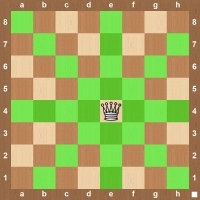
\includegraphics{queen_attack.jpg}
                        \centering
                \end{figure}
		The N-queen problem is a generalization of normal chess queen problem, which is an 8-queen problem. \\
		Also, it is proven that N-queen problem is always solvable for $N\neq2,3$. \\
		Time complexity of this problem is $O(N^{N})$, therefore it is worth it to try to use AI to solve the problem.
	\pagebreak
	\section{Comparison of hill climbing algorithms on N-queens}
		Now we are going to compare different algorithms for different queen amounts and different steps. \\
		As a baseline we will take 1000 runs of each algorithm and we will give each algorithm at most 0.1 seconds to complete, after that we will terminate it and take what it had at the moment as a result (all of them are anytime algorithms, so we can do that easily). This will give us quite a bit of runs of every algorithm, but it won't last forever if every instance times out (1000 runs * 0.1 s * 6 algorithms = 600 seconds = 10 minutes of testing in the worst case) of course, we could let them run longer, or more times, but I think this will give us a nice baseline. \\
		The tests are done on a dedicated core of intel i7-9750H processor with 3599.727 cpu MHz and 12288 KB cache size. \\
		Also, since the algorithms check both left and right for the neigbour there is really no need to put max\_step higher than $N/2$ at any point.\\
		Collumn marked xQ,yS means x queens, y maximum allowed steps. RN-random neighbour, RR- random restart, Stoc - stochastic, SA - simulated anneling. All times are in ms.
		\begin{figure}[h!]
			\centering
			\caption{Algorithm test results for 4 queens}
			\begin{tabular}{|c|c|c|c|c|c|c|}
				\hline \hline
				& \multicolumn{3}{c|}{4Q,1S} & \multicolumn{3}{c|}{4Q,2S} \\
				\hline
				&avg. time&avg. cost&succ. \%&avg. time&avg. cost&succ. \% \\
				\hline \hline
				Simple HC&0.008&0.819&36&0.013&0.358&65.6 \\
				\hline
				Steep HC&0.011&0.669&41.1&0.021&0.308&69.5 \\
				\hline
				RN HC&0.051&0&100&0.047&0&100 \\
				\hline
				RR HC&0.022&0&100&0.020&0&100 \\
				\hline
				Stoc HC&0.050&0&100&0.045&0&100 \\
				\hline
				SA&0.021&0&100&0.024&0&100 \\
				\hline
			\end{tabular}
		\end{figure}
                \begin{figure}[h!]
                        \centering
                        \caption{Algorithm test results for 8 queens}
                        \begin{tabular}{|c|c|c|c|c|c|c|}
                                \hline \hline
                                & \multicolumn{3}{c|}{8Q,2S} & \multicolumn{3}{c|}{8Q,4S} \\
                                \hline
                                &avg. time&avg. cost&succ. \%&avg. time&avg. cost&succ. \% \\
                                \hline \hline
				Simple HC&0.059&1.852&5&0.112&1.311&13.4 \\
                                \hline
				Steep HC&0.105&1.796&4.7&0.214&1.293&12.9 \\
                                \hline
				RN HC&69.784&0.519&48.1&64.779&0.509&49.1 \\
                                \hline
				RR HC&1.300&0&100&0.807&0&100 \\
                                \hline
				Stoc HC&7.001&0&100&6.996&0&100 \\
                                \hline
				SA&34.047&0.344&65.8&4.348&0.037&96.3 \\
                                \hline
                        \end{tabular}
                \end{figure}
                \begin{figure}[h!]
                        \centering
                        \caption{Algorithm test results for 12 queens}
                        \begin{tabular}{|c|c|c|c|c|c|c|}
                                \hline \hline
                                & \multicolumn{3}{c|}{12Q,3S} & \multicolumn{3}{c|}{12Q,6S} \\
                                \hline
                                &avg. time&avg. cost&succ. \%&avg. time&avg. cost&succ. \% \\
                                \hline \hline
				Simple HC&0.343&2.51&0.6&0.539&1.807&4.8 \\
                                \hline
				Steep HC&0.776&2.47&1&1.302&1.728&4.3 \\
                                \hline
				RN HC&98.665&2.112&1.5&95.670&1.642&4.5 \\
                                \hline
				RR HC&37.307&0.098&90.2&12.532&0&100 \\
                                \hline
				Stoc HC&96.946&1.031&5.8&96.394&0.991&7.3 \\
                                \hline
				SA&36.084&0.289&71.6&5.590&0.018&98.2 \\
                                \hline
                        \end{tabular}
                \end{figure}
                \begin{figure}[h!]
                        \centering
                        \caption{Algorithm test results for 20 queens}
                        \begin{tabular}{|c|c|c|c|c|c|c|}
                                \hline \hline
                                & \multicolumn{3}{c|}{20Q,5S} & \multicolumn{3}{c|}{20Q,10S} \\
                                \hline
                                &avg. time&avg. cost&succ. \%&avg. time&avg. cost&succ. \% \\
                                \hline \hline
				Simple HC&2.202&3.463&0&4.156&2.348&2 \\
                                \hline
				Steep HC&7.325&3.515&0.2&14.706&2.24&1.6 \\
                                \hline
				RN HC&100.131&3.423&0.3&99.478&2.22&1.6 \\
                                \hline
				RR HC&96.420&1.112&7.5&80.476&0.627&37.8 \\
                                \hline
				Stoc HC&100.017&3.978&0&100.017&3.961&0 \\
                                \hline
				SA&37.431&0.132&86.8&19.002&0.004&99.6 \\
                                \hline
                        \end{tabular}
                \end{figure}
                \begin{figure}[h!]
                        \centering
                        \caption{Algorithm test results for 30 queens}
                        \begin{tabular}{|c|c|c|c|c|c|c|}
                                \hline \hline
                                & \multicolumn{3}{c|}{30Q,7S} & \multicolumn{3}{c|}{30Q,15S} \\
                                \hline
                                &avg. time&avg. cost&succ. \%&avg. time&avg. cost&succ. \% \\
                                \hline \hline
				Simple HC&10.313&4.589&0&20.891&2.814&0.9 \\
                                \hline
				Steep HC&47.554&4.625&0&97.389&3.082&0.6 \\
                                \hline
				RN HC&101.489&4.549&0&103.645&3.078&0.6 \\
                                \hline
				RR HC&101.458&2.601&0.2&101.606&1.596&2.3 \\
                                \hline
				Stoc HC&100.033&8.485&0&100.034&8.481&0 \\
                                \hline
				SA&76.025&0.466&54.1&62.356&0.254&74.6 \\
                                \hline
                        \end{tabular}
                \end{figure}
		\begin{figure}[h!]
                        \centering
                        \caption{Algorithm test results for 50 queens}
                        \begin{tabular}{|c|c|c|c|c|c|c|}
                                \hline \hline
                                & \multicolumn{3}{c|}{50Q,12S} & \multicolumn{3}{c|}{50Q,25S} \\
                                \hline
                                &avg. time&avg. cost&succ. \%&avg. time&avg. cost&succ. \% \\
                                \hline \hline
				Simple HC&87.415&5.813&0&128.989&3.538&0.3 \\
                                \hline
				Steep HC&114.841&38.295&0&116.458&46.412&0 \\
                                \hline
				RN HC&114.893&38.295&0&116.251&46.412&0 \\
                                \hline
				RR HC&108.736&5.574&0&128.97&3.538&0.3 \\
                                \hline
				Stoc HC&100.092&18.865&0&100.091&18.842&0.9 \\
                                \hline
				SA&99.9564&2.562&0.6&99.872&2.316&1.4\\
                                \hline
                        \end{tabular}
                \end{figure}
		\clearpage
		What are some conclusions we can draw from this? 
		\begin{enumerate}
			\item All of the algorithms will work in a trivial amount of time for 4 queens, since the problem is really easy
			\item Simple and steepest HC will never have 100\% success rate because they consider local optima and shoulders good enough, they don't even try to get out of them
			\item Increasing maximum step increases success chances for every single algorithm: the more neighbours we have to choose from, the better we climb (we can choose better states to go to)
			\item Interestingly enough, increasing maximum step doesn't negatively impact every algorithm, it impacts simple and steepest, but even then the increase in success rate and average cost reduction is well worth it
			\item Increasing maximum step actually decreases average execution time of the rest of the algorithms, probably because, even though neighbour amount is higher the amount of decrease in "wondering" the algoritham does outweighs it.
			\item Increasing the queen amount, logically, makes all algorithms perform worse, but stochastic and random neighbour take the biggest hit (stochastic has a lot more places to wonder to, while random neighbour has a lot of places to get stuck at)
			\item The two algorithms that survived the most and that gave  best results are Random restart and Simulated anneling (with Simulated anneling giving decent results while all others start giving terrible results)
			\item If I had to rank the algorithms I would put Simulated anneling as $1^{st}$, Random restart at $2^{nd}$, Simple HC at $3^{rd}$. The worse one, in my opinion, is Random neighbour, timing out even at low amount of queens. 
		\end{enumerate}
	\clearpage
	\section{Literature}
	\begin{itemize}
		\item \url{https://www.javatpoint.com/hill-climbing-algorithm-in-ai}
		\item \url{https://en.wikipedia.org/wiki/Hill\_climbing}
		\item \url{https://www.thechesswebsite.com/chess-pieces/}
		\item \url{https://en.wikipedia.org/wiki/Eight\_queens\_puzzle}
		\item The Algorithm Design Manual, Skiena, Steven S.
	\end{itemize}
\end{document}	
